% \AtBeginSection[]{
%     \begin{frame}
%         \frametitle{}
%         \tableofcontents[currentsection]
%     \end{frame}
% }

%%%%%%%%%%%%%%%%%%%%%%%%%%%%%%%%%%%%


\subsection{Overview}

\begin{frame}{AOMEA: Assisted MAS Organization Engineering Approach}{Overview}

    \begin{columns}

        \hspace{-7ex}
        \begin{column}{0.5\textwidth}

            \centering
            \vspace{-23.5ex}
            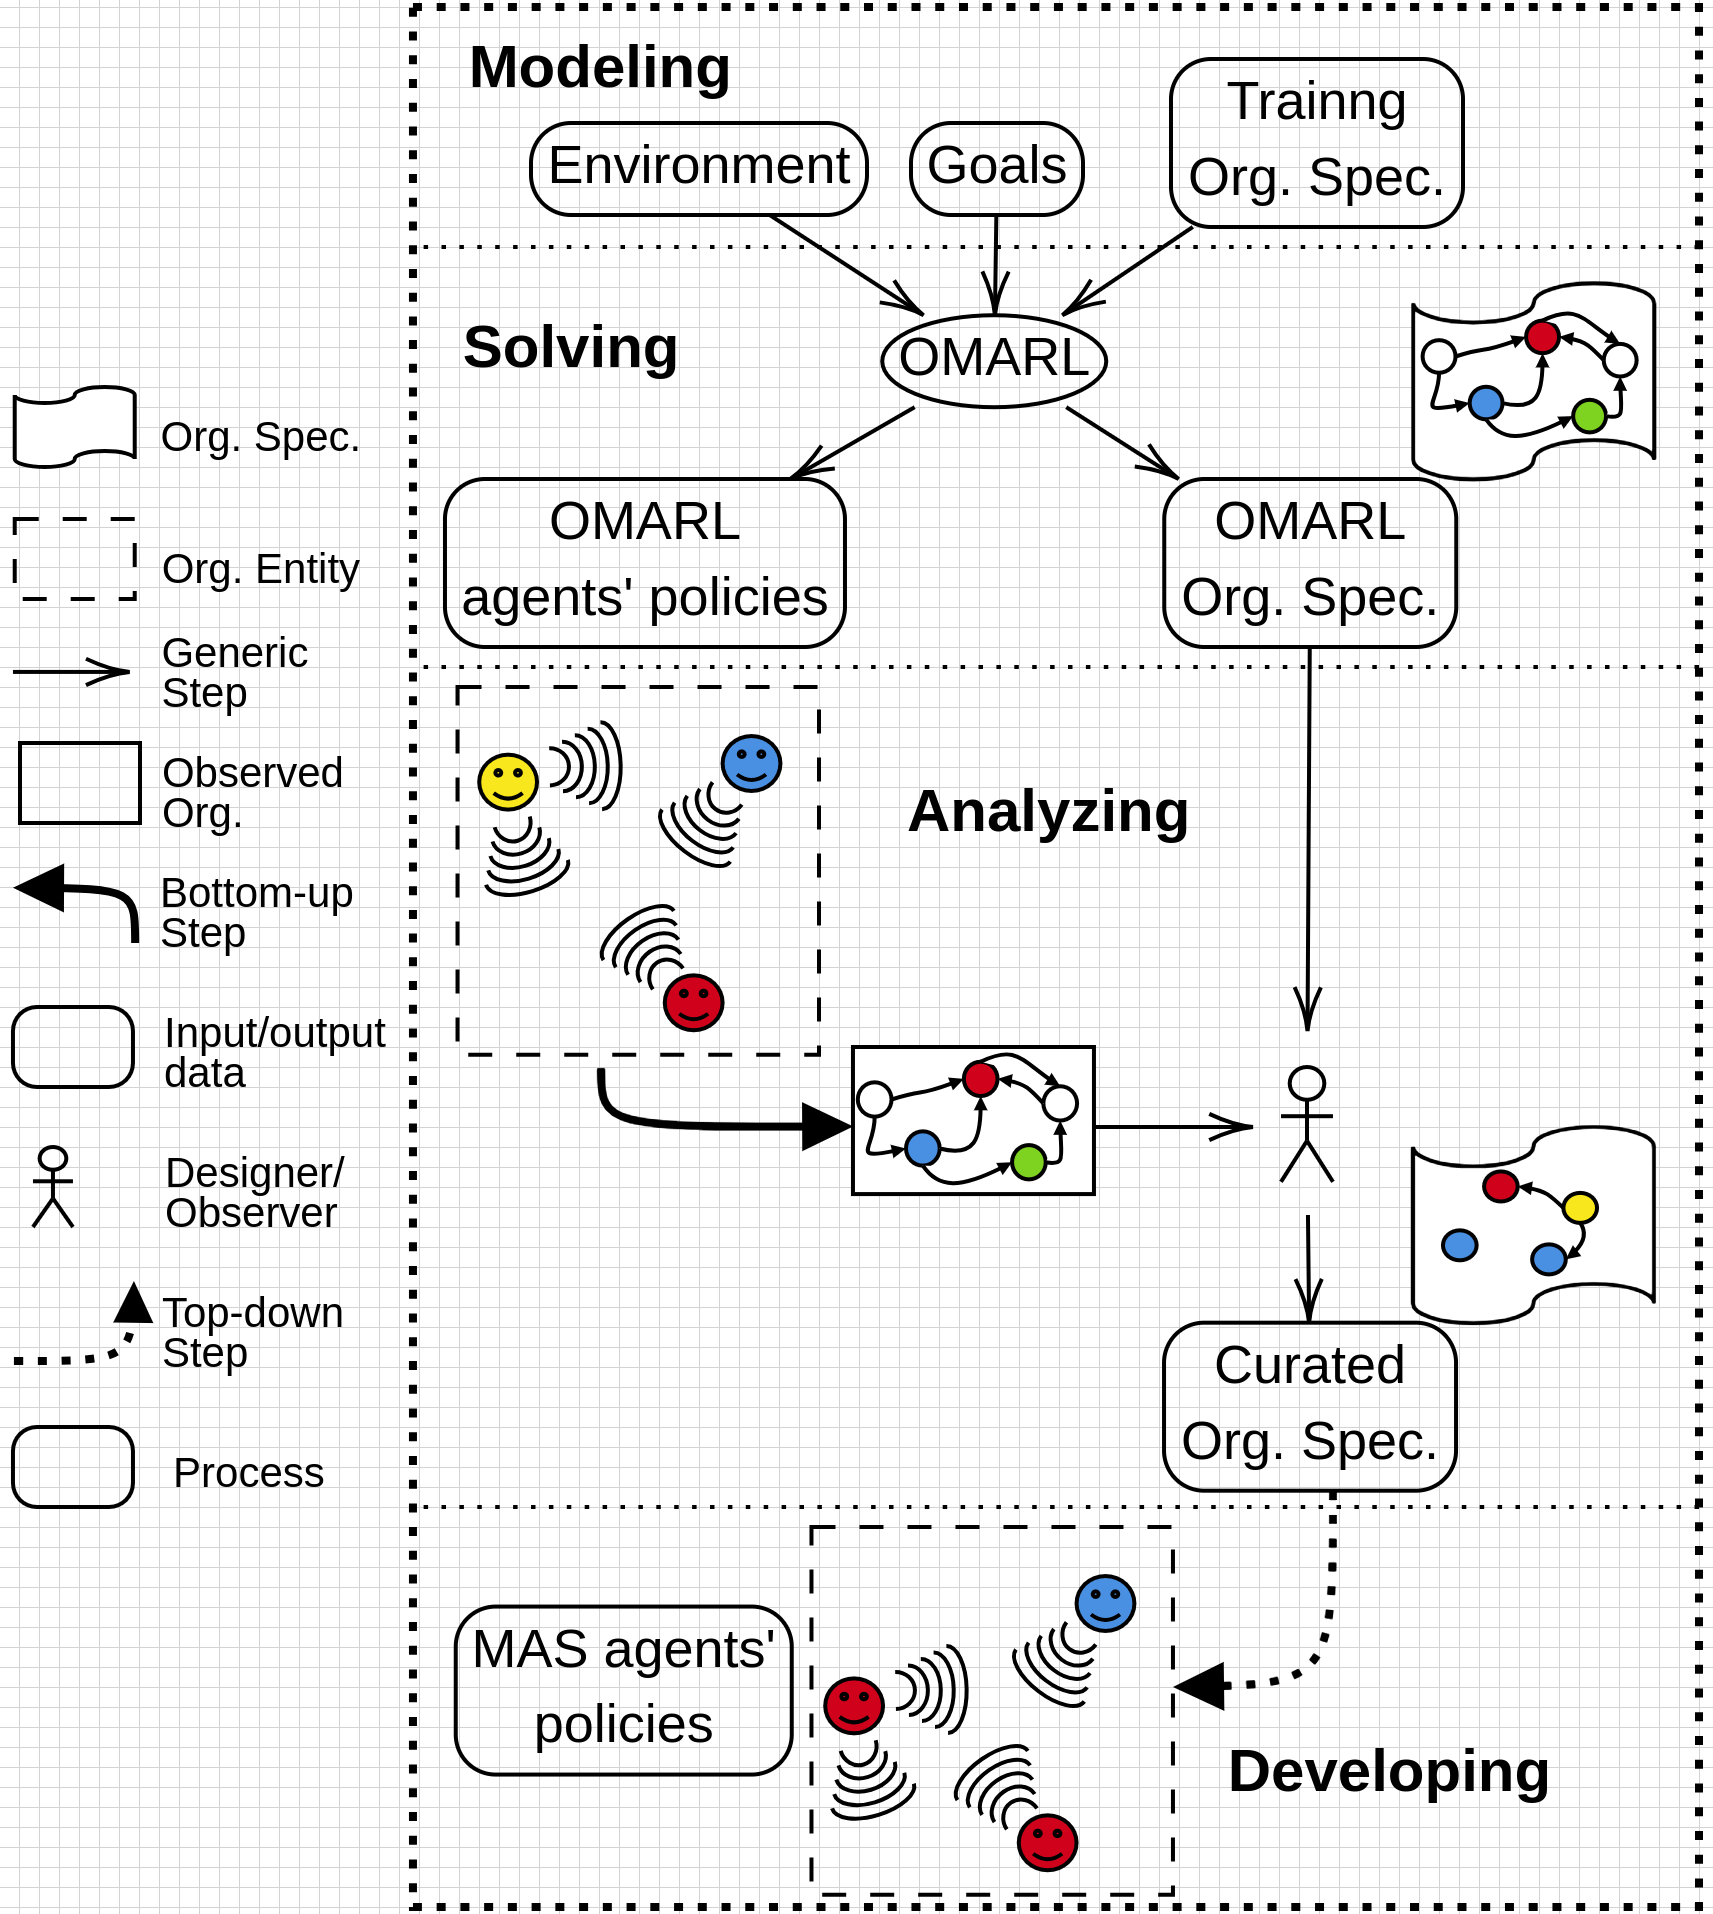
\includegraphics[width=0.95\linewidth]{figures/AOMEA_illustrative_global_view.png}

        \end{column}

        \hspace{-5ex}
        \begin{column}{0.5\textwidth}
            {\small \textbf{Implementing OMARL} $\rightarrow$ \textbf{PRAHOM} \\ { \footnotesize Partial Relations with Agent History and Organization Model}}

            \centering
            \begin{figure}
                \vspace{-4ex}
                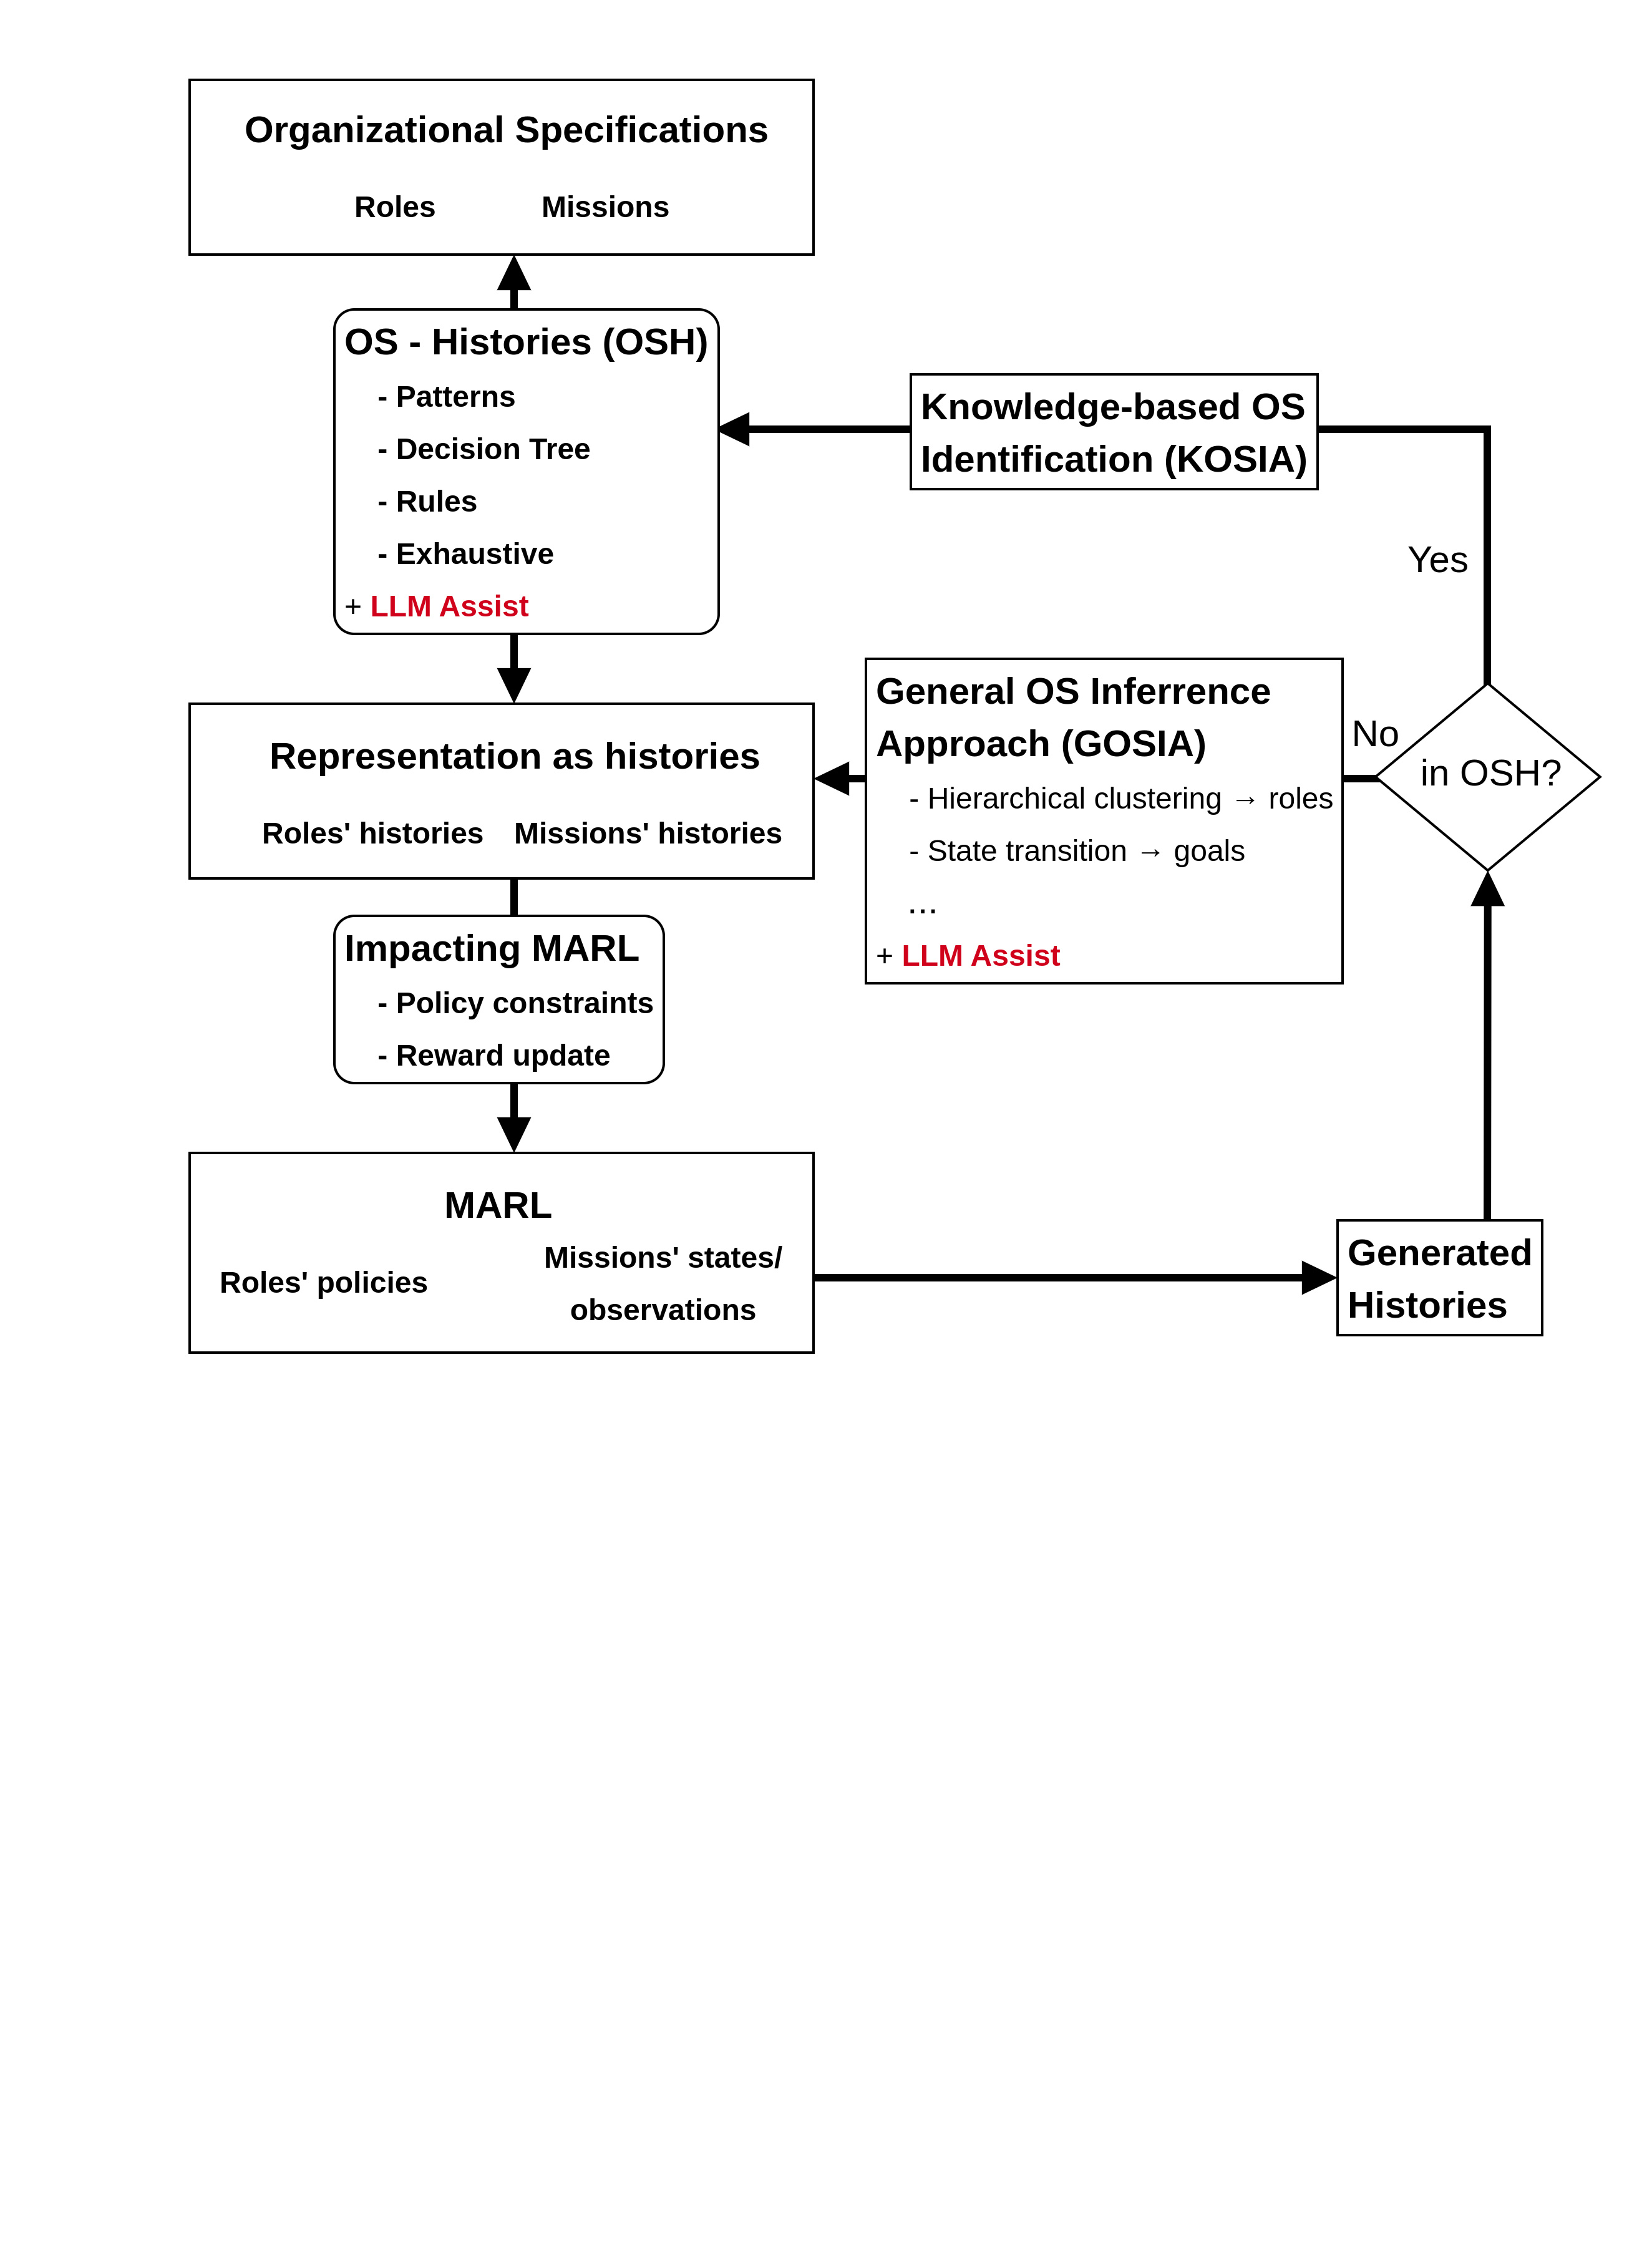
\includegraphics[width=1.1\linewidth]{figures/prahom_overview.png}
            \end{figure}

        \end{column}

    \end{columns}

\end{frame}


\subsection{Engineering tool}

\begin{frame}[fragile]{AOMEA: Assisted MAS Organization Engineering Approach}{Engineering tool}

    \begin{block}{\emph{PRAHOM PettingZoo Wrapper}\label{PettingZoo-wrapper}}
        \begin{itemize}
            \item Uses \textbf{PettingZoo}: standardized API facilitating the application of MARL algorithms;
            \item Proposed as a tool to help the application of \emph{PRAHOM} for a given PettingZoo environment.
        \end{itemize}
    \end{block}

    \begin{lstlisting}[language=Python,basicstyle=\scriptsize]
    from prahom_wrapper import prahom_wrapper
    pz_env = raw_pz_env() ; pz_env = prahom_wrapper(pz_env)
    
    pz_env.train_under_constraints(
        obs_act_to_labels=oal,
        constraint_integration_mode="CORRECT",algorithm_configuration="default_MAPPO"
        osh_model_constraint=osh_model(
            
            structural_specifications=ss(roles={"role_0": history_subset(pattern="[o0,a1](1,4),[o1,a2](1,2)")},role_inheritance_relations=None, root_groups=None),
            
            functional_specifications=fs(social_scheme=sch(goals={"goal_0": history_subset(pattern="[#Any](0,*),[obs_goal_0]")},missions=["mission_0"], goals_structure=None,mission_to_goals={"mission_0": ["goal_0"]},mission_to_agent_cardinality=None),social_preferences=None),

            deontic_specifications={"role_0": {("mission_0", "Any"): ["agent_0", "agent_4"]}}))

    pz_env.generate_organizational_specifications(use_kosia=False, use_gosia=True,gosia_configuration={"generate_figures": True})
    \end{lstlisting}

\end{frame}
